\documentclass[letterpaper, 11pt]{article}
\usepackage{graphicx}	% For figures
\usepackage{natbib}	% For citet and citep
\usepackage{amsmath}	% for \iint
\usepackage{bbm}	% for blackboard bold numbers
\usepackage[left=3cm,top=3cm,right=3cm]{geometry}

\renewcommand{\topfraction}{0.85} \renewcommand{\textfraction}{0.1} 
\parindent=0cm
\newcommand{\sparse}{\texttt{Sparse}}
\newcommand{\cluster}{\texttt{Cluster}}
\newcommand{\crowded}{\texttt{Crowded}}

\title{Probabilistic Catalogs from Crowded Star Fields}
\author{Brendon J. Brewer$^{1, 2, ^*}$, David W. Hogg$^{3}$,
and Daniel Foreman-Mackey$^{3}$ \\
\\
\small
$^1$ Department of Physics, University of California, Santa Barbara,\\
\small
CA 93106, USA \\
\small
$^2$ Department of Statistics, The University of Auckland,\\
\small
Private Bag 92019, Auckland 1142, New Zealand \\
\small
$^3$ Center for Cosmology and Particle Physics, Department of Physics,
New York University,\\
\small
4 Washington Place, New York, NY, 10003, USA\\
\small
$^*$\texttt{bj.brewer@auckland.ac.nz}
}

\begin{document}
\maketitle

\section{Introduction}

A fundamental problem in astronomy is the construction of {\it catalogs} from
raw image data. Essentially, the question being answered is ``given the image
we have obtained, what objects are present in the field and what are their
properties?''.

\section{Probabilistic Catalogs}



\begin{itemize}
\item Catalogs as models for what's out there \\
\item Standard techniques for constructing catalogs, and under what
cicrumstances they stop working \\
\item 
\end{itemize}

\section{The Unknown Parameters}
Our model makes the following assumptions. There are an unknown number of stars
$N$ in the field. Each star has an unknown
position $(x,y)$ in the plane of the sky, and an unknown flux $f$. We also
describe the {\it spatial distribution} of the stars by parameters
$\alpha$, and the distribution of fluxes (commonly known as the {\it luminosity
function}) by parameters $\beta$. In summary, the unknown parameters are:
\begin{eqnarray}
\theta = \left\{N, \alpha, \beta, \left\{x_i, y_i\right\}_{i=1}^N, 
\left\{f_i\right\}_{i=1}^N\right\}
\end{eqnarray}
The prior probability distribution for the unknown parameters can be factorized
using the product rule. With a variety of independence assumptions, the prior
can be written as:
\begin{eqnarray}
p(\theta) = p(N)p(\alpha)p(\beta)\prod_{i=1}^N p(x_i, y_i | \alpha)
p(f_i | \beta) 
\end{eqnarray}
Here, we have assumed that the luminosity function does not depend on position.
We have also assumed independence of $N$, $\alpha$ and $\beta$, which means that
learning the value of one would not tell us anything about the values of the
others. Finally, the positions and fluxes of the stars come independently from
a common distribution. If we knew the spatial distribution and the luminosity
function of the stars, then the location and flux of a particular star would
not tell us anything about the location and flux of another star.

\section{Simulated Data}


A model for the spatial distribution corresponds to a choice of functional
forms for the distributions $p(x_i, y_i | \alpha)$ and $p(f_i | \beta)$.
In this paper we discuss three test cases, named \sparse, \cluster
and \crowded. For the generation of the simulated
images, we used the following assumptions:

\begin{table}
\begin{center}
\begin{tabular}{ccccc}
Test Case & Parameter & Value \\
\hline
\sparse \\
\cluster \\
\crowded
\end{tabular}
\end{center}
\end{table}

\begin{figure}
\hspace{-1cm}
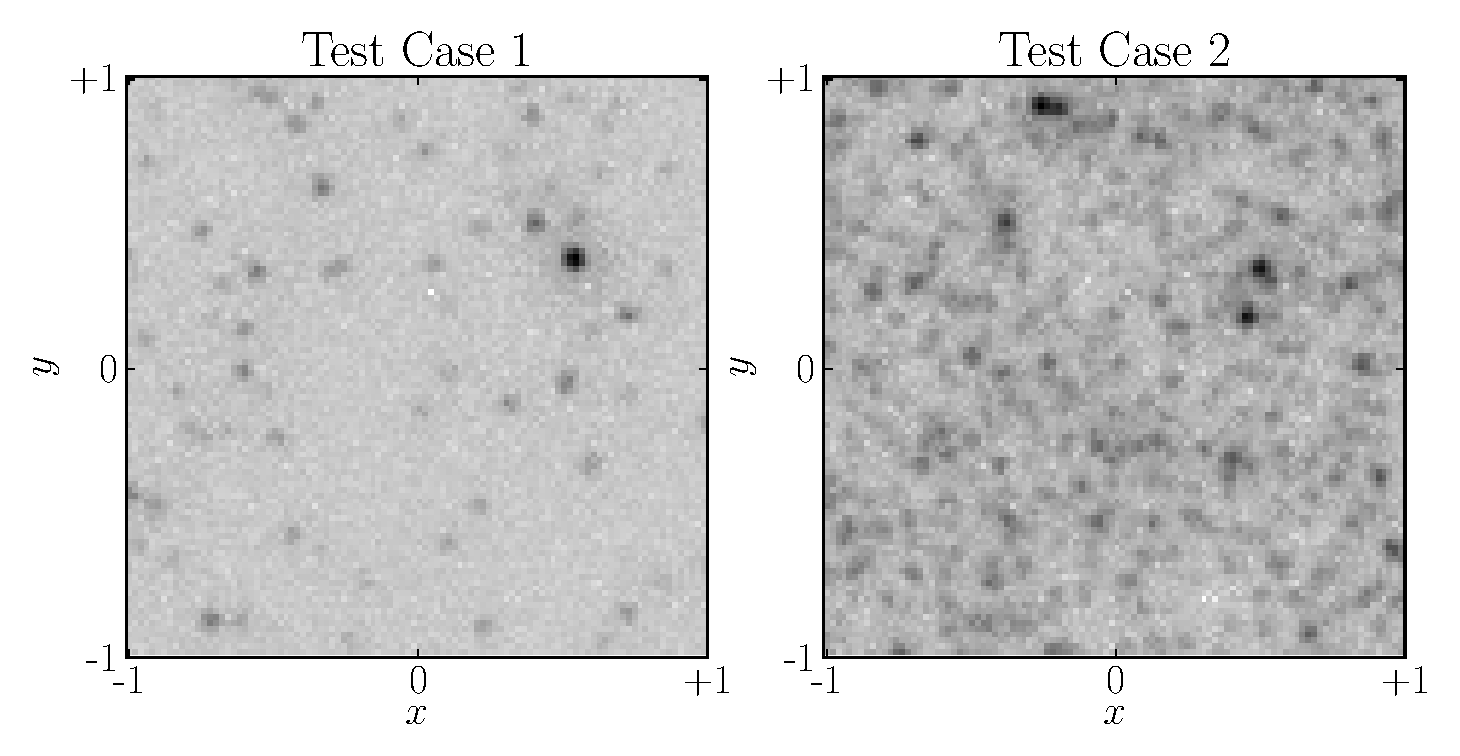
\includegraphics{Figures/test_cases.eps}
\end{figure}

\subsection{Toy Model}
For the first implementation I wrote at NYU, I used the following model and
priors:
\begin{itemize}
\item $N \sim \textnormal{Uniform}(0, 1, 2, ..., 1000)$ \\
\item The parameters of the spatial
distribution: $\alpha = \left\{x_c, y_c, \sigma\right\}$ \\
\item The spatial distribution: $p(x_i, y_i | \alpha)\sim\mathcal{N}\left(
\texttt{mean}=(x_c, y_c), \texttt{covariance}=
\left(\begin{array}{cc}\sigma^2 & 0 \\ 0 & \sigma^2\end{array}\right)\right)$ \\
\item Prior on $\alpha$: Uniform within image for $(x_c, y_c)$, logUniform for
$\sigma$ with max value $\sim$ image size.
\item The luminosity function: $p(f_i | \beta) \sim
\textnormal{Exponential}\left(\texttt{mean}=\beta\right)$ \\
\item Prior on $\beta$: logUniform with generous bounds.
\end{itemize}



\section{A More Realistic Model}
\citep{2008ApJ...682..874K}

\appendix
\section{Pixel Convolved PSF}
Consider a ``true image'' $f_0(x, y)$ with infinite resolution. We now model how
this image gives rise to the observed data. First, it is convolved with a
PSF $g(\delta_x, \delta_y)$ (assumed normalized to 1) to give the blurred image:
\begin{eqnarray}
f_{\rm{blurred}}(x, y) &=& \iint f_0(x-\delta_x, y-\delta_y)
g(\delta_x, \delta_y) \, d\delta_x \, d\delta_y \label{blur}
\end{eqnarray}
Then, we observe the blurred image with a certain pixellation. Consider a pixel.
The true flux $F$ within the pixel is:
\begin{eqnarray}
F &=& \iint_{\rm pixel} f_{\rm blurred}(x, y) \,dx'\,dy'\\
&=& \iint f_{\rm blurred}(x, y)\mathbbm{1}\left[(x,y) \in \textnormal{pixel}
\right] \,dx\,dy \label{pixel}
\end{eqnarray}
Now consider $F$ as a function of the central location $(x_c, y_c)$ of the
pixel.


\section{MCMC Implementation}
\subsection{Current}
I am using Diffusive Nested Sampling \citep{dnest}, which is really just
Metropolis-Hastings but targeting a fancy distribution instead of the actual
posterior, and then assigning importance weights when you want the posterior.
Nested Sampling is good because it is invariant under monotonic transformations
of the likelihood function. i.e. the exploration only depends on things like
whether one point is better than another, and not on how much better it is.

\subsection{Improving the Efficiency of Reversible Jump}
Instead of parameterising by $N$ and the positions and fluxes, what if we have
$3N_{\rm max}$ latent variables $\theta$ that always exist, and transform these
into
positions and fluxes by a transformation $f$:
\begin{eqnarray}
\{\mathbf{x}, \mathbf{y}, \mathbf{f}\} &=& f(\theta)
\end{eqnarray}
The transformation can be parameterized by various parameters of its own, such
that a known fraction of the fluxes end up being nonzero, etc. This could have
various advantages, most notably: when new stars are added, they are added with
low fluxes. It also turns the variable dimension problem into a fixed dimension
one, so emcee, MultiNest or similar will now work, although the multimodality problem will
still exist.

\subsubsection{Proposal Distributions}

\begin{table}
\begin{center}
\begin{tabular}{c|c|c}
Parameter & Proposal & Notes\\
\hline
$N$ & $N \to N + \delta_N$ & Generate $\delta_N$ new stars from prior given
$(\alpha, \beta)$\\
$N$ & $N \to N - \delta_N$ & Remove $\delta_N$ stars at random\\
$\alpha$ & $\alpha \to \alpha + \delta_\alpha$ & Move stars along with $\alpha$
\\
$\alpha$ & $\alpha \to \alpha + \delta_\alpha$ & Stars fixed, use logHastings
factor \\
$\beta$ & $\beta \to \beta + \delta_\beta$ & Move stars' fluxes along with
$\beta$\\
$\beta$ & $\beta \to \beta + \delta_\beta$ & Stars' fluxes fixed, use
logHastings factor \\
$(x,y)$ & $(x,y) \to (x,y)+(\delta_x, \delta_y)$ & Can move $>1$ star.
Include prior via logH \\
$f$ & $f \to f + \delta_f$ & Can move $>1$ stars' fluxes. Include prior
via logH
\end{tabular}
\end{center}
\caption{All $\delta$ parameters are drawn from multi-scale distibutions such
that the largest steps are of order the prior width, and the smallest steps
are of order $10^{-6}$ times the prior width.\label{proposals}}
\end{table}

See Table~\ref{proposals} for a list of current proposal distributions.

%\subsection{Future Possibilities}
%{\bf Hogg}: {\it I think this problem is important enough and general enough
%that we should spend some time working on some ideas there.  If we can sample
%over image explanations, our powers in astronomy will be awesome
%beyond our wildest imaginings.}

%\subsection{Genetic Moves}
%Here I will sketch some ideas...




\begin{thebibliography}{99}
\bibitem[\protect\citeauthoryear{Brewer, P{\'a}rtay, 
\& Cs{\'a}nyi}{2011}]{dnest} Brewer B.~J., P{\'a}rtay L.~B.,
Cs{\'a}nyi G., 2011, Statistics and Computing, 21, 4, 649-656. arXiv:0912.2380

\bibitem[\protect\citeauthoryear{Green}{1995}]{rjmcmc}
Green, P.~J., 1995, Reversible Jump Markov Chain Monte Carlo Computation and Bayesian Model Determination, Biometrika 82 (4): 711–732.

\bibitem[Kelly et al.(2008)]{2008ApJ...682..874K} Kelly, B.~C., Fan, X., 
\& Vestergaard, M.\ 2008, ApJ, 682, 874 

\bibitem[Mackay(2003)]{mackay} Mackay, D.~J.~C., 2003, Information Theory,
Inference and Learning Algorithms, Cambridge University Press, UK.

\bibitem[\protect\citeauthoryear{Skilling}{1998}]{massinf} 
Skilling J., 1998, Massive Inference and Maximum Entropy, in Maximum Entropy 
and Bayesian Methods, Kluwer Academic Publishers, Dordrecht/Boston/London p.14
\end{thebibliography}

\end{document}

